\chapter{Software}
This chapter contains the design choices and an explanation of the different design blocks.

\section{CDU}
The software on the microcontroller governs the sensor communication, the PC communication and the memory. The hierarchy of software can be seen on the class diagram in figure ~\ref{fig:cduclassd}.

\begin{figure}[H]
\centering
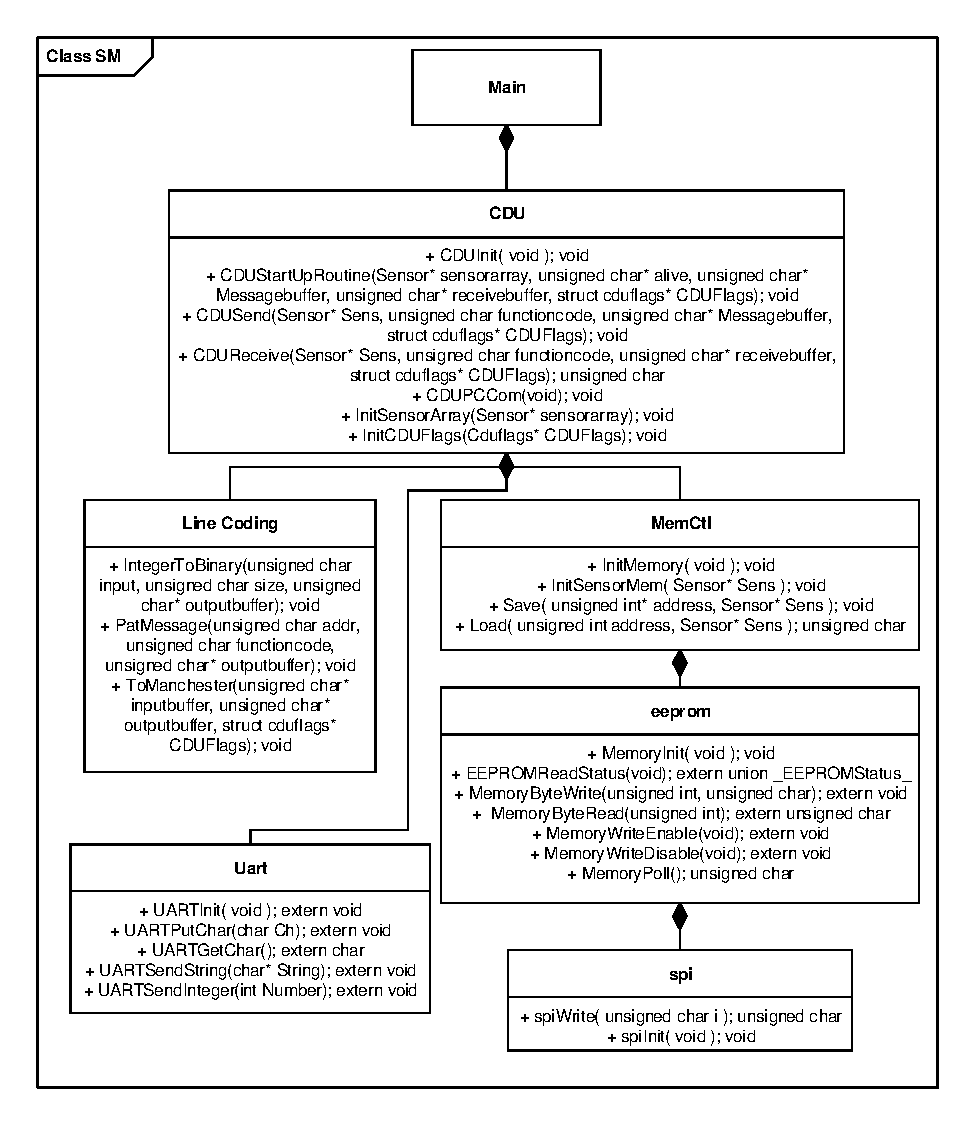
\includegraphics[scale=0.8]{billeder/CDUClassDiagramme}
\label{fig:cduclassd}
\caption{CDU Class diagram}
\end{figure}

\subsection{Variables:}
The global variables in the CDU includes 2 structs. These 2 structs will be shown in their own table.
\begin{table}[H]
\begin{tabular}{|l|p{10cm}|}
\hline
\cellcolor[gray]{0.8}\textbf{Variable} &\cellcolor[gray]{0.8} \textbf{Description}\\ \hline
\texttt{comflag} & This varible(flag) determines whether a message is written on the bus.\\ 
\hline
\texttt{msgflag} & This varible(flag) determines whether a message is ready to be written on the bus.\\ 
\hline
\texttt{clk$\_$flag} & This varible(flag) determines whether to put a low or high out on the bus while not communicating.\\ 
\hline
\texttt{recvflag} & This varible(flag) determines whether a message has been received on the bus.\\ 
\hline
\texttt{enableflag} & This varible(flag) determines when a transmission can be written on the bus.\\ 
\hline
\end{tabular}
\label{tab:structcduflags}
\caption{Struct CDUFlags}
\end{table}

\begin{table}[H]
\begin{tabular}{|l|p{10cm}|}
\hline
\cellcolor[gray]{0.8}\textbf{Variable} &\cellcolor[gray]{0.8} \textbf{Description}\\ \hline
\texttt{Address} & This variable contains the address of the sensor node.\\ 
\hline
\texttt{Data} & This variable contains the data of the sensor node.\\ 
\hline
\texttt{Year} & This variable contains the current year.\\ 
\hline
\texttt{Day} & This variable contains the current day.\\ 
\hline
\texttt{Hour} & This variable contains the current hour.\\ 
\hline
\texttt{Minute} & This variable contains the current minute.\\ 
\hline
\texttt{Errors} & This variable contains the errors explained in the protocol section of the architecture document.\\ 
\hline
\texttt{Type} & This variable contains the type of the sensor node.\\ 
\hline
\end{tabular}
\label{tab:structsensor}
\caption{Struct Sensor}
\end{table}

\begin{table}[H]
\begin{tabular}{|l|p{10cm}|}
\hline
\cellcolor[gray]{0.8}\textbf{Variable} &\cellcolor[gray]{0.8} \textbf{Description}\\ \hline
\texttt{message} & The array will contain messages the are to be written to the bus.\\ 
\hline
\texttt{response} & The array will contain messages that have been read from the bus.\\ 
\hline
\texttt{alive} & The array contains values depending if a sensor is alive or not.\\ 
\hline
\texttt{loopcounter} & This variable(counter) is used for writing to the bus.\\ 
\hline
\texttt{recvcounter} & This variable(counter) is used for reading from the bus.\\ 
\hline
\texttt{waitclock} & This variable(counter) is used for delaying when in between writing to the bus and reading from the bus.\\ 
\hline
\texttt{addresscounter} & This variable(counter) is used for placing the point in memory in the right place.\\ 
\hline
\texttt{maincounter} & This variable(counter) is used for delaying in between transmission sequences.\\ 
\hline
\end{tabular}
\label{tab:globalvar}
\caption{Global variables}
\end{table}


\subsection{Function descriptions:}

\begin{table}[H]
\begin{tabular}{l p{12.5cm}}
\multicolumn{2}{l}{\texttt{\textcolor{blue}{void} CDUInit( \texttt{\textcolor{blue}{void}})}} \\
\hline
Description:& The function is used to Initiate the whole CDU. The proper register settings for timer, uart and spi are set. Arrays and structs are initialised.\\
Parameters:&none\\
Return value:&none\\
\end{tabular}
\end{table}

\begin{table}[H]
\begin{tabular}{l p{12.5cm}}
\multicolumn{2}{p{15cm}}{\texttt{\textcolor{blue}{void} IntegerToBinary( \texttt{\textcolor{blue}{unsigned char} input, \textcolor{blue}{unsigned char} size, \textcolor{blue}{unsigned char*} outputbuffer  }) } } \\
\hline
Description:& The function is used convert an integer to a binary array.\\
Parameters:&\texttt{\textcolor{blue}{unsigned char} input}\\
&\texttt{\textcolor{blue}{unsigned char} size}\\
&\texttt{\textcolor{blue}{unsigned char*} outputbuffer}\\
Return value:&none\\
\end{tabular}
\end{table}

\begin{table}[H]
\begin{tabular}{l p{12.5cm}}
\multicolumn{2}{p{15cm}}{\texttt{\textcolor{blue}{void} PatMessage( \texttt{\textcolor{blue}{unsigned char} addr, \textcolor{blue}{unsigned char} functioncode, \textcolor{blue}{unsigned char*} outputbuffer  }) } } \\
\hline
Description:& The function is used create a message from the start code, an address and a function code. This is put into the outputbuffer.\\
Parameters:&\texttt{\textcolor{blue}{unsigned char} addr}\\
&\texttt{\textcolor{blue}{unsigned char} functioncode}\\
&\texttt{\textcolor{blue}{unsigned char*} outputbuffer}\\
Return value:&none\\
\end{tabular}
\end{table}

\begin{table}[H]
\begin{tabular}{l p{12.5cm}}
\multicolumn{2}{p{15cm}}{\texttt{\textcolor{blue}{void} ToManchester( \texttt{\textcolor{blue}{unsigned char*} inputbuffer, \textcolor{blue}{unsigned char*} outputbuffer, \textcolor{blue}{Cduflags*} CDUFlags  }) } } \\
\hline
Description:& The function is used convert the message contained in the inputbuffer to manchester coding and put it in the outputbuffer. The outputbuffer must be twice the size of the inputbuffer. The cduflags struct contains flags to signal when a message has been put into the outputbuffer.\\
Parameters:&\texttt{\textcolor{blue}{unsigned char*} inputbuffer}\\
&\texttt{\textcolor{blue}{unsigned char*} outputbuffer}\\
&\texttt{\textcolor{blue}{Cduflags*} CDUFlags}\\
Return value:&none\\
\end{tabular}
\end{table}

\begin{table}[H]
\begin{tabular}{l p{12.5cm}}
\multicolumn{2}{l}{\texttt{\textcolor{blue}{void} InitSensorArray( \texttt{\textcolor{blue}{Sensor*} sensorarray})}} \\
\hline
Description:& The function is used to Initiate the sensorarray with addresses and values. Addresses are assigned from 1 to 15. The rest is instantiated to zero.\\
Parameters:&\texttt{\textcolor{blue}{Sensor*} sensorarray}\\
Return value:&none\\
\end{tabular}
\end{table}

\begin{table}[H]
\begin{tabular}{l p{12.5cm}}
\multicolumn{2}{l}{\texttt{\textcolor{blue}{void} InitCDUFlags( \texttt{\textcolor{blue}{Cduflags*} CDUFlags})}} \\
\hline
Description:& The function is used to Initiate the cduflags in the Cduflags struct to zero.\\
Parameters:&\texttt{\textcolor{blue}{Sensor*} sensorarray}\\
Return value:&none\\
\end{tabular}
\end{table}

\begin{table}[H]
\begin{tabular}{l p{12.5cm}}
\multicolumn{2}{p{15cm}}{\texttt{\textcolor{blue}{void} CDUStartUpRoutine( \texttt{\textcolor{blue}{Sensor*} sensorarray, \textcolor{blue}{unsigned char*} alive, \textcolor{blue}{unsigned char*} Messagebuffer, \textcolor{blue}{unsigned char*} receivebuffer, \textcolor{blue}{Cduflags*} CDUFlags})}} \\
\hline
Description:& The function is used to send messages with the GETINFO function code to every sensor in the sensorarray. If a response has been received, the type is stored in the relevant sensor struct in the sensorarray. The alive is updated with the responding sensor.\\
Parameters:&\texttt{\textcolor{blue}{Sensor*} sensorarray}\\
&\texttt{\textcolor{blue}{unsigned char*} alive}\\
&\texttt{\textcolor{blue}{unsigned char*} Messagebuffer}\\
&\texttt{\textcolor{blue}{unsigned char*} receivebuffer}\\
&\texttt{\textcolor{blue}{Cduflags*} CDUFlags}\\
Return value:&none\\
\end{tabular}
\end{table}

\begin{table}[H]
\begin{tabular}{l p{12.5cm}}
\multicolumn{2}{p{15cm}}{\texttt{\textcolor{blue}{void} CDUSend( \texttt{\textcolor{blue}{Sensor*} Sens, \textcolor{blue}{unsigned char} functioncode, \textcolor{blue}{unsigned char*} Messagebuffer, \textcolor{blue}{Cduflags*} CDUFlags})}} \\
\hline
Description:& The function is used to send messages with the function code to the sensor inserted. The cduflags struct is used to poll on when to send and to set the comflag. if a function code larger than 15 is inserted the function sends out function code 0 which will result in an error on the sensor node side.\\
Parameters:&\texttt{\textcolor{blue}{Sensor*} sensorarray}\\
&\texttt{\textcolor{blue}{unsigned char} functioncode}\\
&\texttt{\textcolor{blue}{unsigned char*} Messagebuffer}\\
&\texttt{\textcolor{blue}{Cduflags*} CDUFlags}\\
Return value:&none\\
\end{tabular}
\end{table}

\begin{table}[H]
\begin{tabular}{l p{12.5cm}}
\multicolumn{2}{p{15cm}}{\texttt{\textcolor{blue}{unsigned char} CDUReceive( \texttt{\textcolor{blue}{Sensor*} Sens, \textcolor{blue}{unsigned char} functioncode, \textcolor{blue}{unsigned char*} receivebuffer, \textcolor{blue}{Cduflags*} CDUFlags})}} \\
\hline
Description:& The function is used to receive messages from the receivebuffer and verify address and function code. If the proper address and function code is received data or type is stored in the relevant sensor struct. If verification fails it returns 0. If everything went as expected a 1 is returned. 2 is returned if the function code is larger than 15.\\
Parameters:&\texttt{\textcolor{blue}{Sensor*} sensorarray}\\
&\texttt{\textcolor{blue}{unsigned char} functioncode}\\
&\texttt{\textcolor{blue}{unsigned char*} receivebuffer}\\
&\texttt{\textcolor{blue}{Cduflags*} CDUFlags}\\
Return value:&\texttt{\textcolor{blue}{unsigned char} errors}\\
\end{tabular}
\end{table}

\section{Sensor node}